\chapter{Data Mining}
\begin{figure}[ht!]
    \centering
    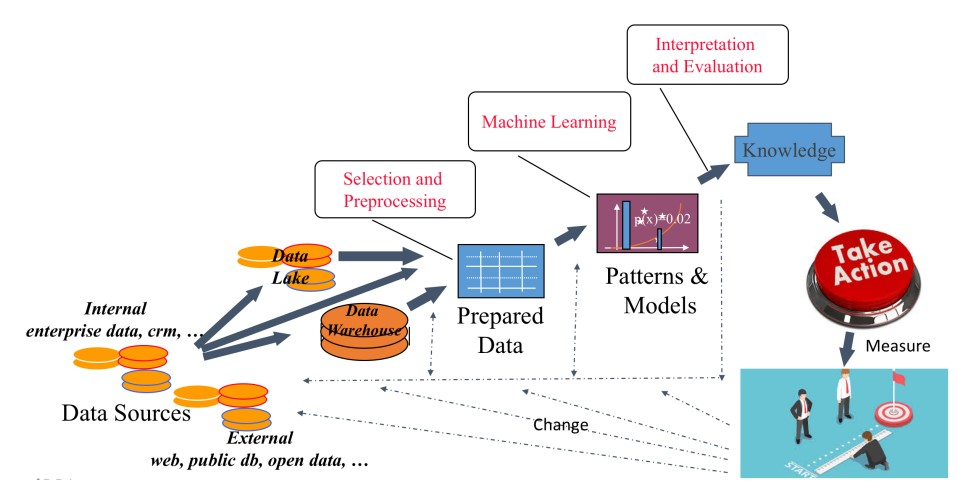
\includegraphics[scale=0.52]{images/Data_Mining_process.jpg}
    \caption{The Data Mining Process}
\end{figure}

\textbf{\textit{Data Mining}} is the process of discovering patterns, trends, correlations, or meaningful information from large datasets. It involves the application of various techniques from \textit{statistics}, \textit{machine learning}, and \textit{database systems} to extract valuable knowledge from raw data.

\section{Business Intelligence and Data Warehouses}

\paragraph{Business Intelligence (BI)}
\textbf{\textit{Business Intelligence (BI)}} represents a key concept in the field of Data Mining and can be described as the process of:
\begin{itemize}
    \item transforming raw data into useful information to support effective and aware business strategies
    \item capturing the business data and getting the right information to the right \textit{people}, at the right \textit{time}, through the right \textit{channel}.
\end{itemize}
There are different definition that has been provided during the years, but there are two of them in particular that we can highlight:
\begin{quote}
    \textit{Business intelligence (BI) is an umbrella term that includes the applications, infrastructure and tools, and best practices that enable access to and analysis of information to improve and optimize decisions and performance. - \textbf{Gartner}}
\end{quote}
\begin{quote}
    \textit{Business Intelligence is a set of methodologies, processes, architectures, and technologies that transform raw data into meaningful and useful information used to enable more effective strategic, tactical, and operational insights and decision-making. - \textbf{Forrester Research}}
\end{quote}

\paragraph{Data Warehouse (DWH)}
One of the main tools to support BI is the \textbf{\textit{Data Warehouse (DWH)}}, which is a type of \textit{Decision Support System (DSS)} and can be seen informally as an optimized repository that stores information for the decision-making process. With the huge and increasing number of information that companies have to manage in order to find relevant business strategies DWHs answer to the necessity of more sophisticated solutions than classical operational databases.\\
The main advantages are the following:
\begin{itemize}
    \item they provide the ability to manage sets of historical data;
    \item they provide the ability to run multidimensional analysis accurately and rapidly;
    \item they are based on a simple model that can be easily learned by its users;
    \item they are the basis for indicator-calculating systems.
\end{itemize}

More formally, we can say that a \textbf{\textit{Data Warehouse (DWH)}} is a specialized database that stores large volumes of historical data and facilitates the analysis and reporting of that data to support \textit{decision-making processes}. It provides several key features:

\begin{itemize}
    \item \textbf{Subject-Oriented:} A data warehouse is designed to focus on specific subjects or domains relevant to the enterprise's operations, such as customers, products, sales, etc. By organizing data around these core concepts, it enables analysts and decision-makers to gain insights into various aspects of the business.

    \item \textbf{Integration and Consistency:} One of the primary functions of a DWH is to integrate data from multiple disparate sources, including transactional databases, spreadsheets, and external systems. This integration ensures that data from different sources is harmonized and provides a unified view across the organization. Consistency in data representation and structure is maintained to ensure accuracy and reliability in analysis.

    \item \textbf{Evolution Over Time and Non-Volatility:} A crucial aspect of a data warehouse is its ability to capture and track changes in data over time. Historical data are preserved, allowing for the analysis of trends and patterns spanning various time periods. Unlike transactional databases where data may be constantly updated or overwritten, data in a data warehouse are non-volatile. Once committed, the data remains static, read-only, and preserved for future reporting and analysis.

\end{itemize}

In summary, a \textbf{\textit{DWH}} serves as a centralized repository for historical data, providing a comprehensive and consistent view of the organization's information assets. By offering subject-oriented, integrated, and non-volatile data, it empowers decision-makers with valuable insights for strategic planning, performance analysis, and informed decision-making.

\paragraph{Data Mart (DM)}
A \textbf{Data Mart (DM)} serves as a specialized subset or aggregation of the data stored within a primary DWH. Unlike the comprehensive nature of a DWH, a \textbf{DM} contains a focused set of information tailored to \textit{meet the needs of a specific business area}, corporate department, or category of users.

One of the key roles of \textbf{DMs} is to act as building blocks during the incremental development of DWHs. Rather than attempting to construct an entire DWH in one go, organizations often adopt an iterative approach, creating smaller, more \textit{targeted DMs} that address immediate business needs. As the organization's analytical requirements evolve, additional DMs can be added or expanded upon, gradually contributing to the development of a comprehensive DWH architecture.

Moreover, \textbf{DMs} help to address the users' queries more efficiently. By tailoring the data content and structure to align with the analytical needs of particular departments or user categories, DMs facilitate more efficient and focused analysis. This granularity enables users to access and analyze relevant data without being overwhelmed by the vast volume of information typically found in a primary DWH.

Furthermore, \textbf{DMs} often offer improved performance compared to primary DWHs. Due to their smaller size and targeted scope, DMs can deliver faster query response times and better overall system performance. By focusing on specific subsets of data, data marts reduce the complexity of queries and minimize the processing overhead associated with accessing and retrieving information.

\begin{figure}[ht!]
    \centering
    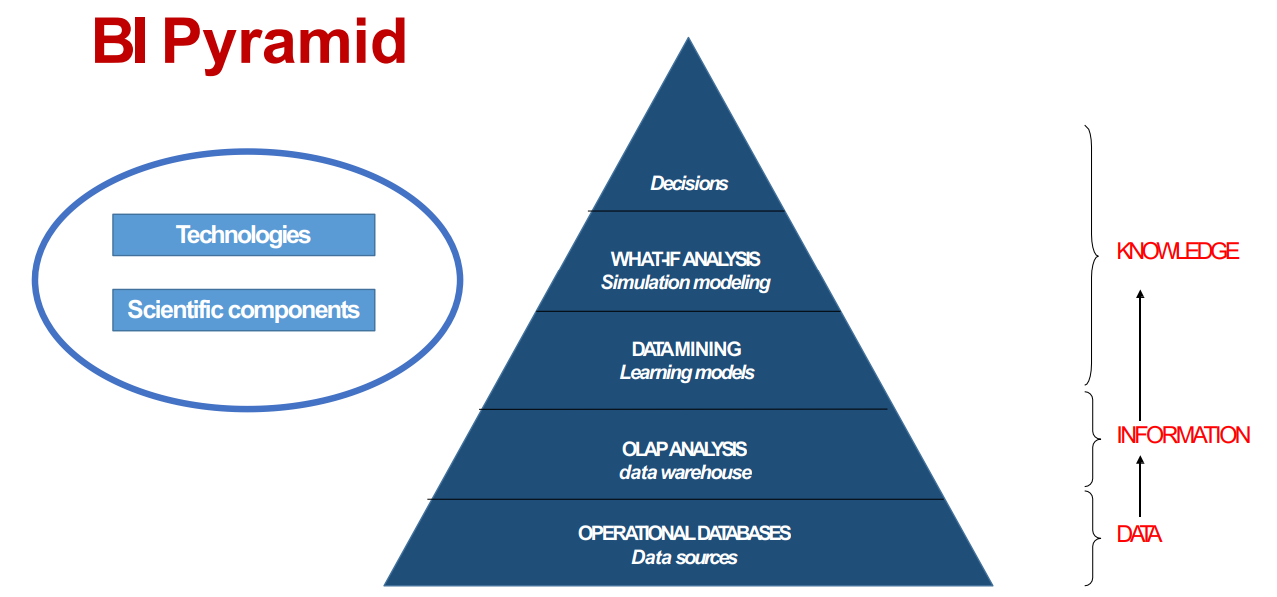
\includegraphics[scale=0.39]{images/BI_pyramid.png}
\end{figure}

\subsection{Online Analytical Processing (OLAP)}

First of all, data are organised in \textbf{tables}, which are defined as collections of related, homogeneous data arranged into a row-column format, which includes:
\begin{itemize}
    \item \textbf{Rows:} the various components stored in the table about a \textit{specific individual};
    \item \textbf{Columns:} the type and the meaning of a \textit{specific component} of the individuals represented in the table;
    \item \textbf{Key:} a column or a set of columns whose values allow to distinguish \textit{univocally} the rows of the table.
\end{itemize}

\textbf{\textit{On-Line Analytical Processing (OLAP)}} allows users  to interactively navigate the data warehouse information exploiting the multidimensional model, providing a flexible and intuitive way to explore, query, and report on large datasets. Typically, the data are analyzed at different levels of aggregation, by applying subsequent \textit{\textbf{OLAP operators}}, each yielding one or more different queries.

In an \textbf{OLAP Session} the user can scout the multidimensional model choosing the next operator based on the outcome of the previous ones. In this way, the user creates a navigation path that corresponds to an analysis process for facts according to different points and at different detail levels.
\begin{quote}
    \centering
    \textit{Product} $\longrightarrow$ \textit{Sub-Category} $\longrightarrow$ \textit{Category}
\end{quote}

The \textbf{OLAP operators} are the following:
\begin{itemize}
    \item \textbf{Roll-up:} causes an increase in data aggregation and removes a detail level from a hierarchy by collapsing the rows that have a feature in common.
    \begin{figure}[ht!]
        \centering
        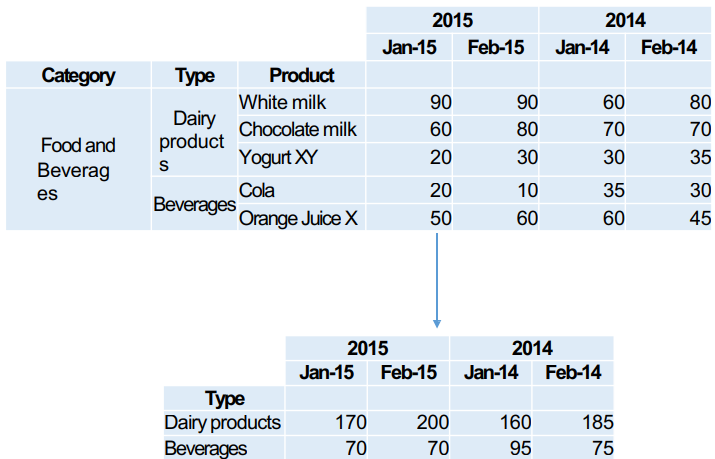
\includegraphics[scale=0.55]{images/OLAP_roll_up.png}
    \end{figure}
    \item \textbf{Drill-down:} is the complement to the roll-up operator; it reduces data aggregation and adds a new detail level to a hierarchy (e.g., from category to subcategory).
    \begin{figure}[ht!]
        \centering
        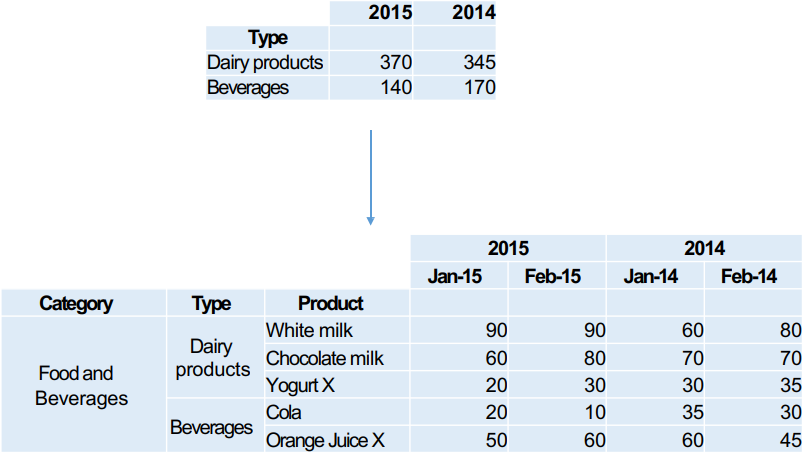
\includegraphics[scale=0.55]{images/OLAP_drill_down.png}
    \end{figure}
    \item \textbf{Slice-and-dice:} the \textit{slicing} operation reduces the number of cube dimensions after setting one of the dimensions to a specific value (e.g., category = 'Food and Beverages'); the \textit{dicing} operation reduces the set of data being analysed by a selection criterion.
    \begin{figure}[ht!]
        \centering
        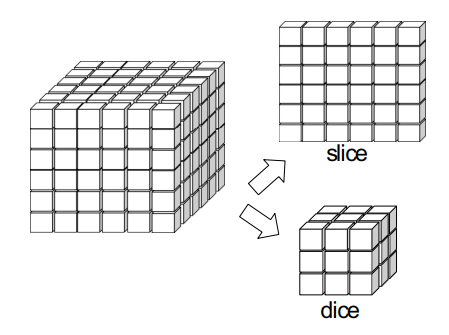
\includegraphics[scale=0.55]{images/OLAP_slice_and_dice.png}
    \end{figure}
    \item \textbf{Pivot:} implies a change in layouts, aiming at analysing a group of data from a different viewpoint.
    \begin{figure}[ht!]
        \centering
        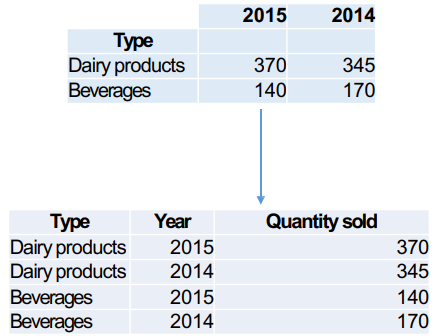
\includegraphics[scale=0.55]{images/OLAP_pivot.png}
    \end{figure}
    \item \textbf{Drill-across:} allows to create a link between concepts in interrelated cubes, in order to compare them.
    \begin{figure}[ht!]
        \centering
        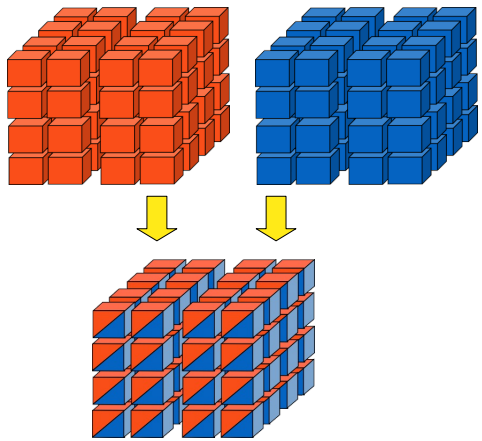
\includegraphics[scale=0.5]{images/OLAP_drill_across.png}
    \end{figure}
    \item \textbf{Drill-through:} switches from multidimensional aggregate data to operational data insources or in the reconciled layer.
    \begin{figure}[ht!]
        \centering
        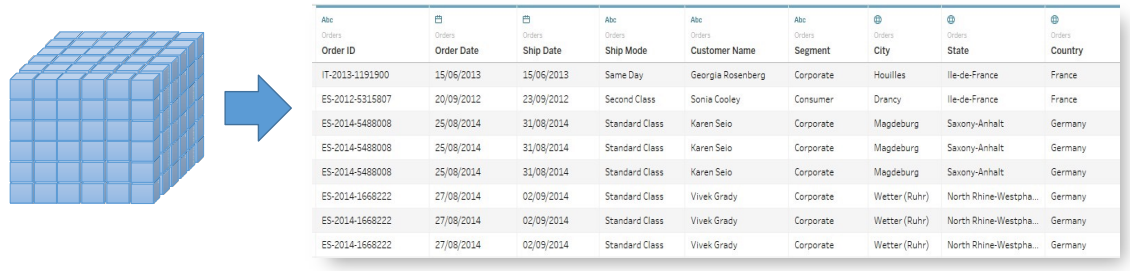
\includegraphics[scale=0.44]{images/OLAP_drill_through.png}
    \end{figure}
\end{itemize}

\subsection{Extraction, Transformation and Loading (ETL)}

The \textit{\textbf{ETL (Extract, Transform, Load)}} process is a crucial component of data warehousing and business intelligence. It involves \textbf{extracting} data from various sources, \textbf{cleansing} them, \textbf{transforming} them into a consistent format, and \textbf{loading} them into a target destination, such as a data warehouse, where they can be analyzed and queried effectively. Let's analyse the single phases.

\subsubsection{Extraction}
In the \textbf{extraction phase}, data (\textit{structured} or \textit{unstructured}) is collected from multiple disparate sources, including databases, flat files, APIs, and external systems. The methods used for this process vary depending on the source systems and the nature of the data:
\begin{itemize}
    \item \textbf{Static extraction:} retrieving all the data from the source. Used to populate the data warehouse for the first time.
    \item \textbf{Incremental extraction:} updating the data warehouse regularly only with the data that have been modified. In this case data comes with an associated \textit{timestamp} and \textit{triggers} (related to change transactions for relevant data).
    \item \textbf{Real-Time extraction:} continous stream of data.
\end{itemize}

\subsubsection{Cleansing}
This phase is about all those procedures to improve the \textbf{quality} of the retrieved data, by standardizing it and correcting \textbf{mistakes} like \textit{duplicate or missing data}, \textit{unexpeted use of some fields}, \textit{impossible or wrong values} and \textbf{inconsistences} due to \textit{different practices used} or \textit{typing mistakes}. Each type of problem requires different techniques for its solution. We can distinguish three main techniques:
\begin{figure}[ht!]
    \centering
    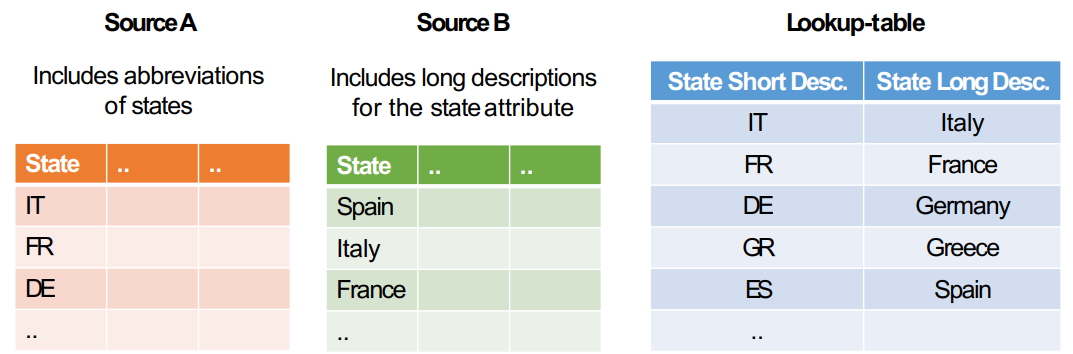
\includegraphics[scale=0.34]{images/ETL_dict_based_techniques.png}
    \caption{Format discrepancies}
    \label{figDictBasedTec}
\end{figure}
\begin{itemize}
    \item \textbf{Dictionary-based techniques:} they are used to check the correctness of the attribute values based on \textit{lookup tables} and \textit{dictionaries} to search for abbreviations and synonyms. We can apply these techniques if the domain is known and limited. These techniques are suitable for typing mistakes and format discrepancies [Figure \ref{figDictBasedTec}, \ref{figDictBasedTec2}].
    \begin{figure}[ht!]
        \centering
        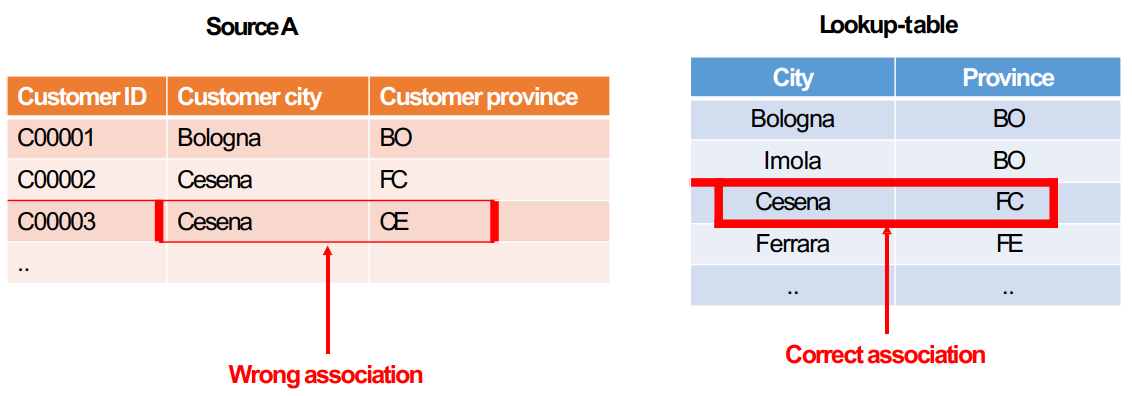
\includegraphics[scale=0.43]{images/ETL_dict_based_techniques_2.png}
        \caption{Inconsistences between correlated attributes}
        \label{figDictBasedTec2}
    \end{figure}
    \item \textbf{Approximate merging:} we use this technique when we need to merge data coming from different sources and we don't have a common key to identify matching tuples:
    \begin{itemize}
        \item \textit{Approximate join} - comparing records from different datasets using similarity measures or matching algorithms to identify potentially related records. (?)
        \begin{figure}[ht!]
            \centering
            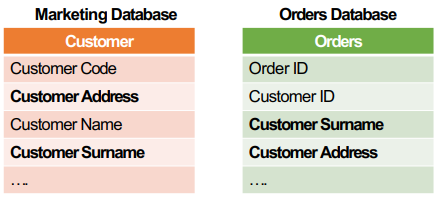
\includegraphics[scale=0.9]{images/ETL_approximate_join.png}
            \caption{Approximate join on \textit{Customer Address} and \textit{Customer Surname}}
        \end{figure}
        \item \textit{Similary functions} - usage of \textbf{affinity functions} (Levenshtein distance, Jaccard similarity, etc.) to compute the similarity between two words and if the result is higher/lower than a treshold, then the two words are the same and the rows can be merged. 
        \begin{figure}[ht!]
            \centering
            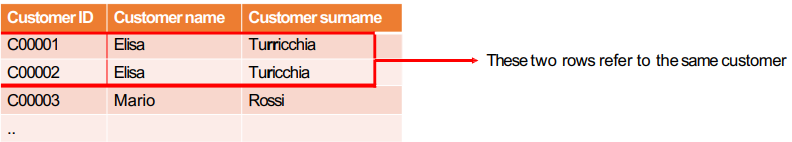
\includegraphics[scale=0.78]{images/ETL_similarity_functions.png}
        \end{figure}
    \end{itemize}
    \item \textbf{Ad-hoc algorithms:} custom algorithms based on specific business rules.
\end{itemize}

\subsubsection{Transformation}
In this phase, data from sources is properly transformed to adjust its format to the reconciled schema. It includes:
\begin{itemize}
    \item \textbf{Conversion:} changes on data
    types and format, like:
    \begin{itemize}
        \item \textit{date conversion}: from date to number (e.g. 12/11/2018 $\longrightarrow$ 20181112)
        \item \textit{string conversion}: lowercase to uppercase (e.g. unibo $\longrightarrow$ UNIBO)
        \item \textit{naming convention transformation}: short description to long
        description (e.g. IT $\longrightarrow$ Italy)
    \end{itemize}
    \item \textbf{Enrichment:} combination of one or more attribute to create new information, like derived data (e.g. Profit = Receipts - Expenses).
    \item \textbf{Separation/Concatenation:} attributes concatenation (e.g. customer surname $\Vert$ customer name)
    \item \textbf{Denormalization/Normalization:} organization of data in tables, where each piece appears only once for normalization and introduction of small redundancy to improve query performance. Typically, in the DWH the data is \textit{denormalized}.
    \begin{figure}[ht!]
        \centering
        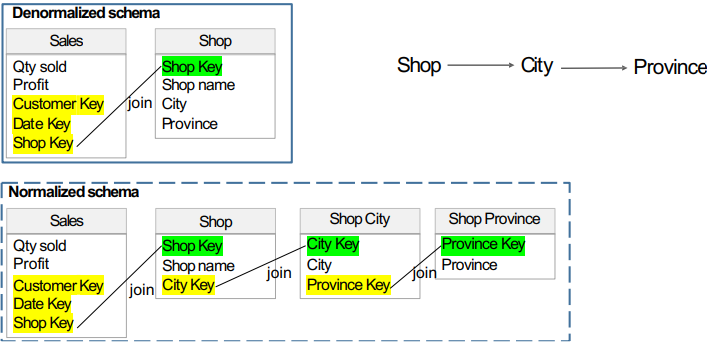
\includegraphics[scale=0.8]{images/ETL_denormalization.png}
        \caption{Denormalization process}
    \end{figure}
\end{itemize}

\subsubsection{Loading}
This is the phase of loading data into a DWH, which can be done in batches or in real-time, depending on the volume of data. During the loading process, data integrity and consistency are maintained to ensure that the data remains accurate and usable for analysis. There are two ways of approaching this phase:
\begin{itemize}
    \item \textbf{Refresh:} the DWH is completely rewritten (i.e. older data is replaced). It's used in combination with static extraction.
    \item \textbf{Update:} only those changes applied to source data are added to the DWH. Preexisting data is not deleted or modified. It's used in combination with incremental extraction to regularly update the DWH.
\end{itemize}

\subsection{Data Warehouse Architectures}

The requirements that a Data Warehouse has to satisfy are the following:
\begin{itemize}
    \item \textbf{Separation:} analytical and transactional processing should be kept apart as much as possible.
    \item \textbf{Scalability:} hardware and software architectures should be easy to upgrade as the data volume, which has to be managed and processed, and the number of users' requirements, which have to be met, progressively increase.
    \item \textbf{Extensibility:} the architecture should be able to host new applications and technologies without redesigning the whole system.
    \item \textbf{Security:} monitoring accesses is essential because of the strategic data stored in data warehouses.
    \item \textbf{Administrability:} DWH management should not be overly difficult.
\end{itemize}

\subsubsection{Single-Layer Architecture}

\begin{wrapfigure}{r}{0.5\textwidth}
    \centering
    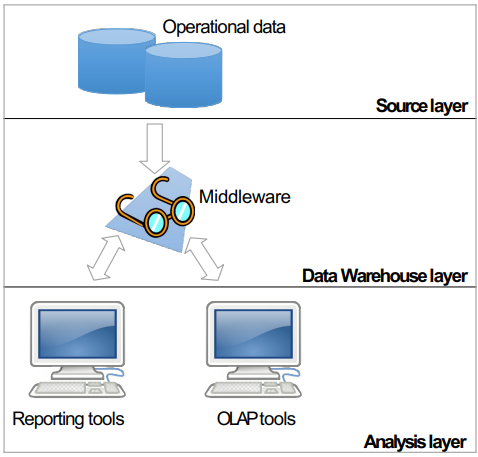
\includegraphics[scale=0.6]{images/DWH_single_layer.png}
\end{wrapfigure}

A \textit{\textbf{Single-Layer architecture}} for a data warehouse provides a straightforward and integrated approach to data storage, processing, and presentation. The source layer is the only physically available layer and its goal is to minimize the amount of data stored, removing data redundancies. DWH is implemented as a multidimensional view of operational data created by specific \textit{middleware}.

Even if this architecture minimizes the space occupation, there is no separation between analytical and transactional processing, which is not ideal for large DWHs and for supporting complex analytical workloads efficiently.

\subsubsection{Two-Layer Architecture}

A \textbf{\textit{Two-Layers architecture}} provides a separation between physically available sources and data warehouses and includes:
\begin{itemize}
    \item \textbf{Source layer:} : it includes a set of heterogeneous data sources (both \textit{internal} and \textit{external sources})
    \item \textbf{Data staging:} the data stored to sources should be extracted, cleansed to remove inconsistencies and fill gaps, and integrated to merge heterogeneous sources into one common schema. It includes \textit{Extraction, Transformation and Loading (ETL)} procedures.
    \item \textbf{Data Warehouse layer:} information is stored to one logically centralized single repository that can be directly accessed or it can be used as source for creating \textit{data marts}. \textit{Meta-data repositories} then store information on sources, data staging, data mart schemata, etc.
    \item \textbf{Analysis layer:} it is accessed by end-user to create reports, dashboard, simulate hypothetical business scenarios, etc.
\end{itemize}

\begin{figure}[ht!]
    \centering
    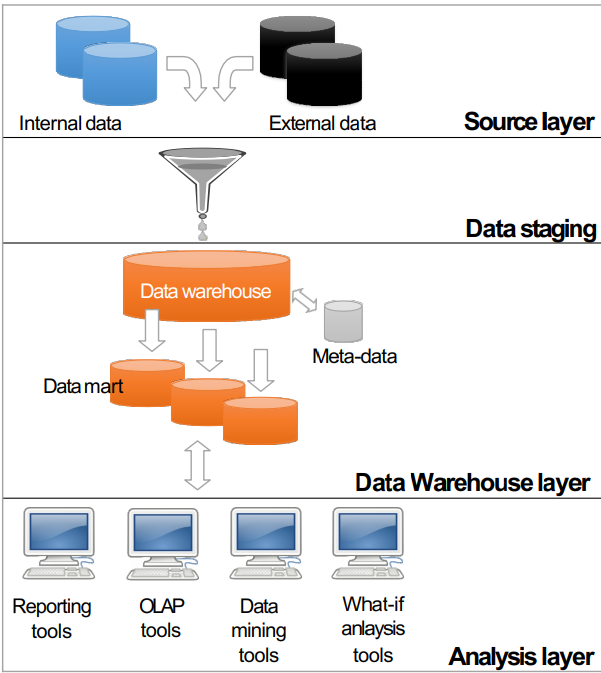
\includegraphics[scale=0.55]{images/DWH_two_layers.png}
\end{figure}

\subsubsection{Three-Layer Architecture}

\begin{wrapfigure}{r}{0.6\textwidth}
    \centering
    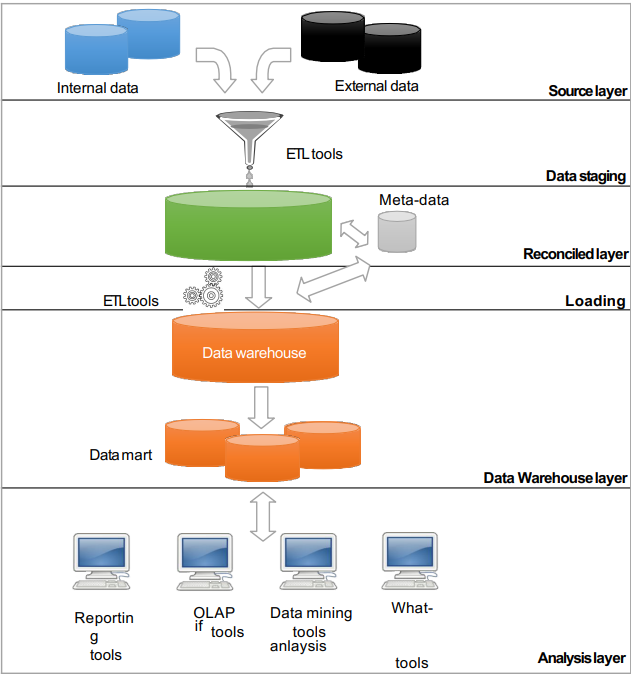
\includegraphics[scale=0.57]{images/DWH_three_layers.png}
\end{wrapfigure}

In a \textbf{\textit{Three-Layers architecture}} the layers are the same as described in the previous case, with one difference:
\begin{itemize}
    \item \textbf{Reconciled layer:} this layer materializes operational data obtained after integrating and cleansing source data. The result data are integrated, consistent, correct, current and detailed.
\end{itemize}

Then, the reconciled data layer creates a common reference data model for a whole enterprise and it separates the problems of source data extraction and integration from those of data warehouse population. In addiction, the reconciled data leads to more redundancy of operational source data.

\subsection{Conceptual Modeling: The Dimensional Fact Model (DFM)}

\textbf{Conceptual modeling} is about creating a high-level representation of a data mining problem that serves as a blueprint to design and implement the solutions, through a framework that guides the entire process. Basically, we have three approaches:
\begin{figure}[ht!]
    \centering
    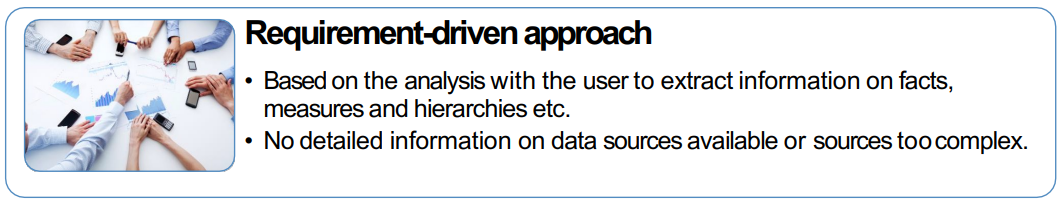
\includegraphics[scale=0.4]{images/conceptual_modeling_1.png}
\end{figure}
\begin{figure}[ht!]
    \centering
    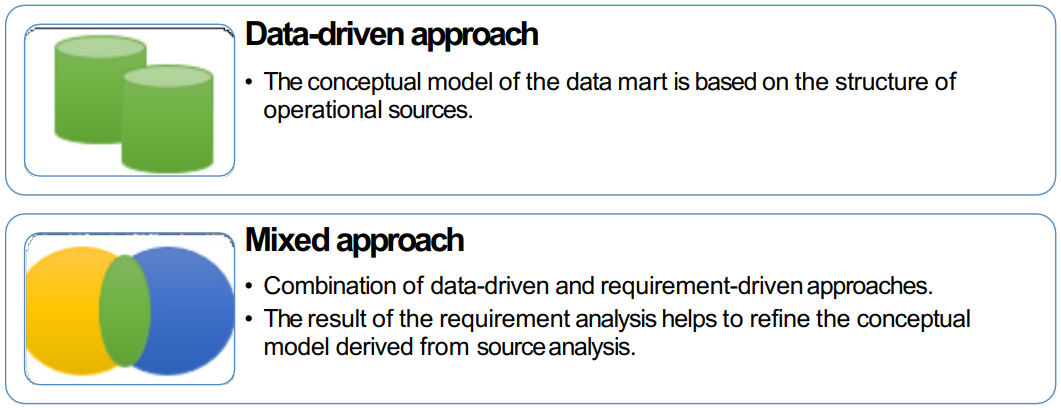
\includegraphics[scale=0.4]{images/conceptual_modeling_2.png}
\end{figure}

The \textbf{\textit{Dimensional Fact Model (DFM)}} is a conceptual model created specifically to function as \textit{data mart design support} in order to emphasize simplicity, flexibility and ease to use for end-users. It is graphic and based on the multidimensional model. Its aim is to:
\begin{itemize}
    \item provide support to conceptual design;
    \item create an environment in which user queries may be formulated intuitively;
    \item favor communication between designers and end users to formalize requirement specifications;
    \item build a stable platform for logical design;
    \item provide clear and effective design documentation.
\end{itemize}

The entire model is deigned around some key concepts:
\begin{center}
    \begin{tabular}{ p{0.17\textwidth} | p{0.5\textwidth} | p{0.33\textwidth}}
        \textbf{Fact} & It is a concept relevant to decision-making processes. It typically models a set of events taking place within a company. & Sales, purchases \\[1.2cm]
        \textbf{Measure} & It is a numerical property of a fact and describes a quantitative fact aspect that is relevant to analysis. & Quantity, discount \\[1.2cm]
        \textbf{Dimension} & It is a fact property with a finite domain and describes an analysis coordination. & Date, product, store \\[0.8cm]
        \textbf{Dimensional attribute} & Dimensions and other possible attributes, always with discrete values, that describe them. & Category of product \\[1.2cm]
        \textbf{Hierarchy} & It is a directed tree whose nodes are dimensional attributes and whose arcs model many-to-one associations between dimensional attribute pairs. It includes a dimension, positioned at the tree's root and all of the dimensional attributes that describe it. & Date $\rightarrow$ Month $\rightarrow$ Year \\[2.5cm]
        \textbf{Primary event} & It is a particular occurrence of a fact, identified by on n-ple made up of a value for each dimension. A value for each measure is associated with each primary event. & 
    \end{tabular}
    \begin{tabular}{ p{0.17\textwidth} | p{0.5\textwidth} | p{0.33\textwidth}}
        \textbf{Secondary event} & Given a set of dimensional attributes, each n-ple of their values identifies a secondary event that aggregates all of the corresponding primary events. Each secondary event is associated with a value for each measure that sums up all the values of the same measure in the corresponding primary events. & 
    \end{tabular}
\end{center}

\begin{figure}[ht!]
    \centering
    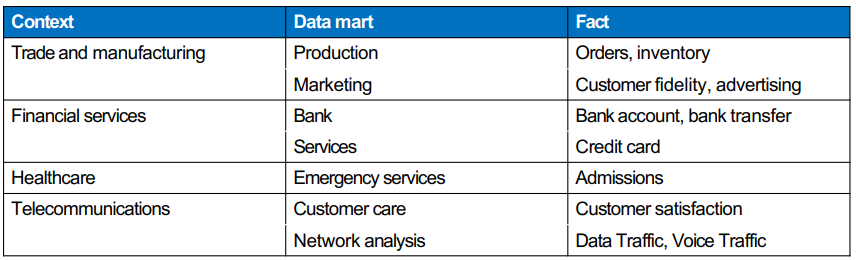
\includegraphics[scale=0.7]{images/DFM_DM_facts.png}
    \caption{Examples of data marts and related facts}
    \label{figDMfacts}
\end{figure}

\begin{figure}[ht!]
    \centering
    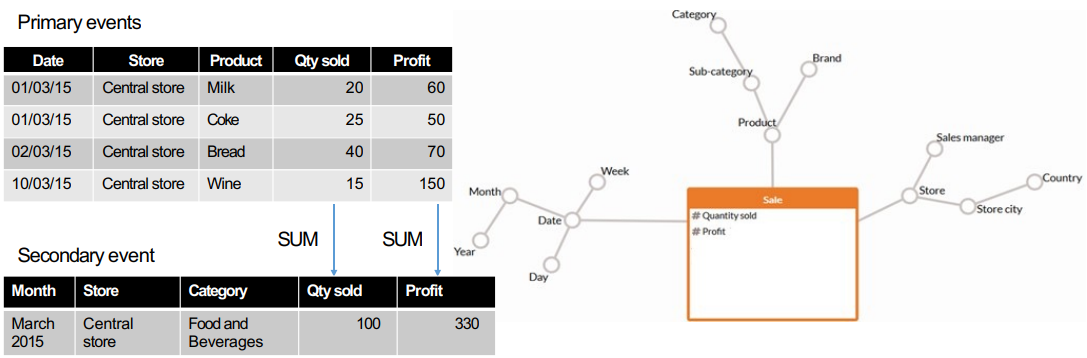
\includegraphics[scale=0.65]{images/DFM_prim_sec_events.png}
    \caption{Examples of primary and secondary events}
    \label{figPrimSecEvents}
\end{figure}

\textit{\textbf{Aggregation}} requires the definition of a suitable \textit{operator} to compose the measure values that mark primary events into values to be assigned to secondary events. Measures are classified into:
\begin{itemize}
    \item \textbf{Flow measures:} refer to a timeframe, at the end of which they are evaluated cumulatively (e.g. quantity sold).
    \item \textbf{Level Measures:} are evaluated at particular times (e.g. number of products ininventory).
    \item \textbf{Unit measures:} are evaluated at particular times but are expressed inrelative terms (e.g. unit price).
\end{itemize}
A measure is called \textbf{additive} along a dimension when you can use the \textit{SUM operator} to aggregate its values along the dimension hierarchy. If this is not the case, it is called \textbf{non-additive}. A non-additive measure is \textbf{non-aggregable} when you can use no aggregation operator for it.
\newpage
\begin{figure}[ht!]
    \centering
    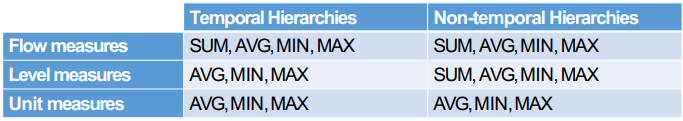
\includegraphics[scale=0.92]{images/DFM_measures.png}
\end{figure}
Given these measures, we can apply different types of \textit{aggregation operators}, as shown in the figure above:
\begin{itemize}
    \item \textbf{Distributive:} calculating aggregates from partial aggregates (e.g. SUM, MIN, MAX).
    \begin{figure}[ht!]
        \centering
        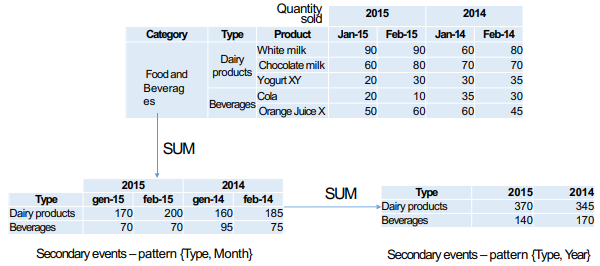
\includegraphics[scale=0.8]{images/DFM_distributive_operator.png}
    \end{figure}
    \item \textbf{Algebraic:} requiring the usage of additional information in the form of a finite number of support measures to correctly calculate aggregates from partial aggregates (e.g. AVG).
    \begin{figure}[ht!]
        \centering
        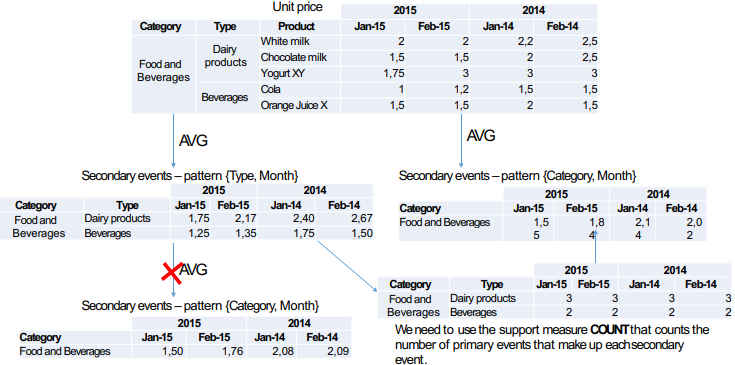
\includegraphics[scale=0.8]{images/DFM_algebraic_operator.png}
    \end{figure}
    \item \textbf{Holistic:} calculating aggregates from partial aggregates only via an infinite number of support measures (e.g. RANK).
\end{itemize}

In addiction to the base attributes, we also have some advanced ones:
\begin{itemize}
    \item \textbf{Descriptive attributes:} used to give additional information to specific dimensional attributes, but they are not used as aggregation criteria.
    \begin{figure}[ht!]
        \centering
        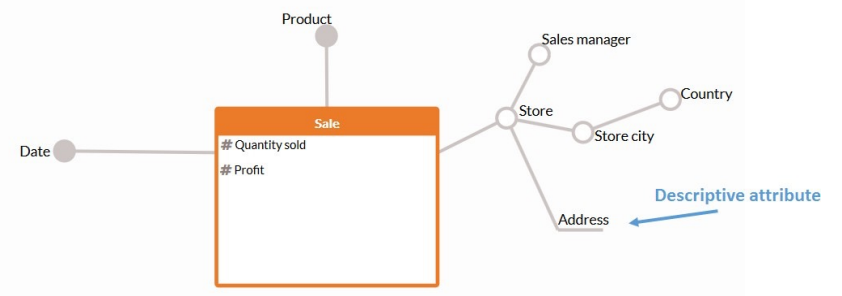
\includegraphics[scale=0.66]{images/DFM_descriptive_attributes.png}
    \end{figure}
    \item \textbf{Cross-dimensional attributes:} a dimensional or descriptive attributes whose value is defined by the combination of two or more dimensional attributes, possibly belonging to different hierarchies.
    \begin{figure}[ht!]
        \centering
        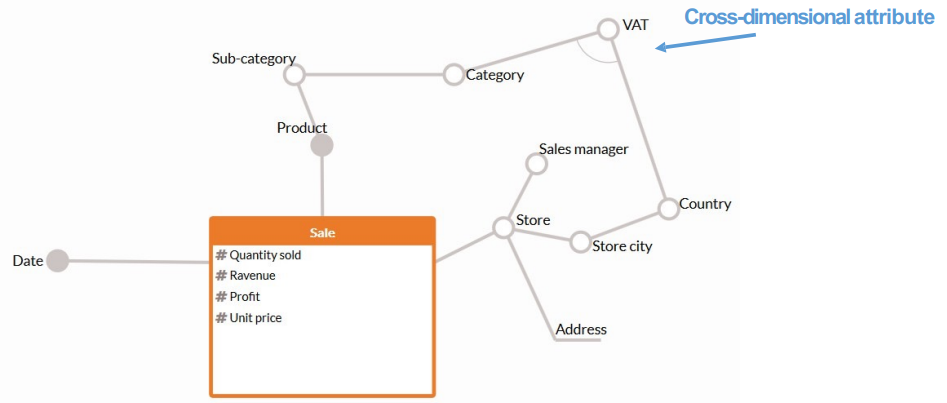
\includegraphics[scale=0.65]{images/DFM_cross_dimensional_attributes.png}
    \end{figure}
    \item \textbf{Convergence:} Two or more arcs belonging to the same hierarchy and ending at the same dimensional attribute.
    \begin{figure}[ht!]
        \centering
        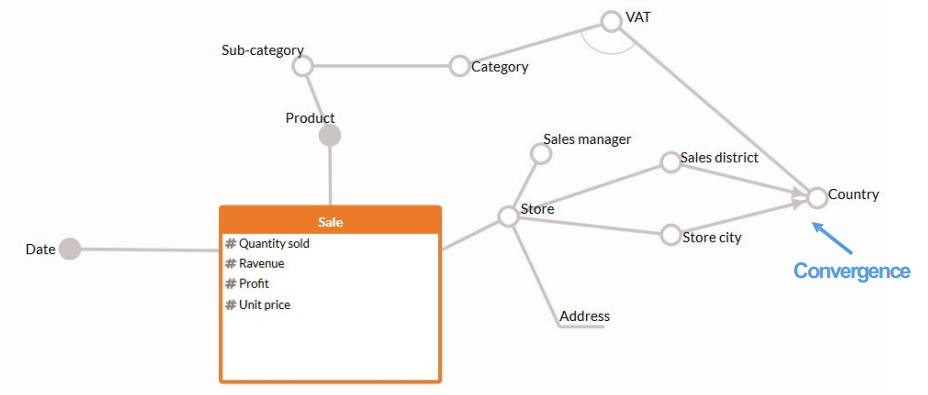
\includegraphics[scale=0.65]{images/DFM_convergence.png}
    \end{figure}
    \item \textbf{Shared hierarchies:} a double circle represents and emphasizes the first attribute to be shared (e.g., City). All descendants of the shared attribute are shared, too. For each incoming arc a role must be added (e.g. customer's city).
    \begin{figure}[ht!]
        \centering
        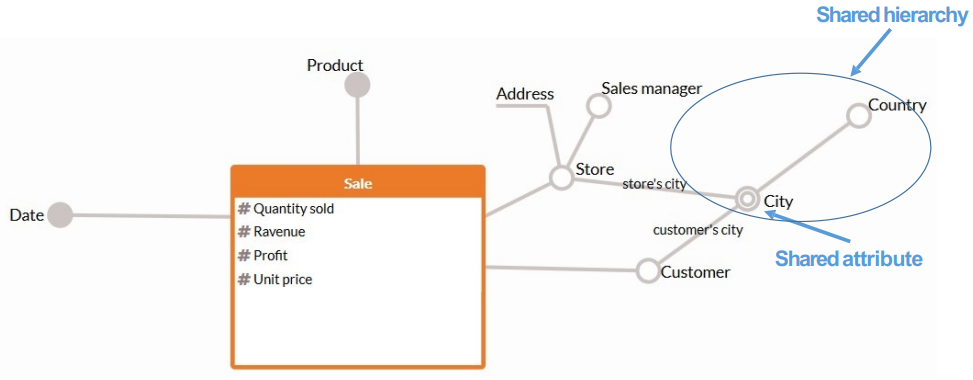
\includegraphics[scale=0.7]{images/DFM_shared_hierarchies.png}
    \end{figure}
    \item \textbf{Multiple arcs:} the meaning of a multiple arc that goes from an attribute called \textit{a} (e.g., book) to an attribute called \textit{b} (e.g., author) is that a many-to-many association exists between \textit{a} and \textit{b}.
    \begin{figure}[ht!]
        \centering
        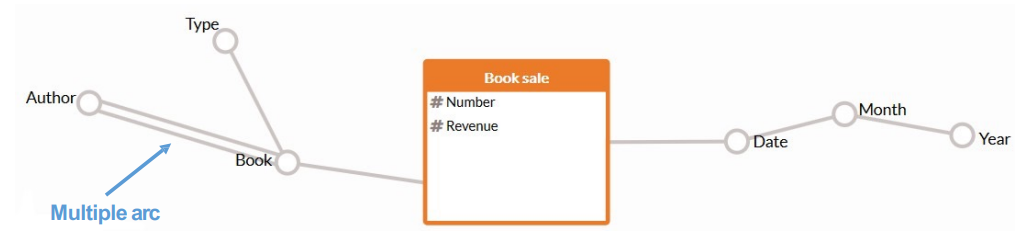
\includegraphics[scale=0.65]{images/DFM_multiple_arcs.png}
    \end{figure}
    \item \textbf{Optional arcs:} used to model scenarios for which an association represented in a fact schema is not defined for a subset of events.
    \item \textbf{Coverage:} when two or more optional arcs exit from the same attribute \textit{a} (e.g., Product), you can specify their coverage:
    \begin{itemize}
        \item the coverage is \textit{\textbf{total}} if the value of at least one of the children is linked to each value of \textit{a}. If, instead, values of \textit{a} exist for which all of the children are undefined, the coverage is \textit{\textbf{partial}}.
        \item the coverage is \textit{\textbf{disjoint}} if you have a value for at most one of the children corresponding to each value of \textit{a}. If, instead, values of \textit{a} exist linking to values of two or more children, the coverage is \textit{\textbf{overlapping}}.
    \end{itemize}
    \begin{figure}[ht!]
        \centering
        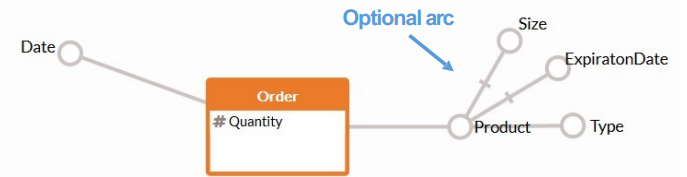
\includegraphics[scale=0.8]{images/DFM_optional_arcs_coverage.png}
    \end{figure}
    \item \textbf{Incomplete hierarchies:} one in which one or more levels of aggregation prove missing in some instances (because they are not known or defined).
    \begin{figure}[ht!]
        \centering
        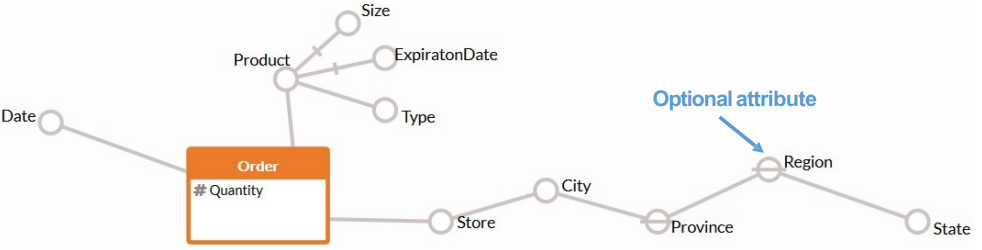
\includegraphics[scale=0.7]{images/DFM_incomplete_hierarchies.png}
    \end{figure}
    \item \textbf{Recursive hierarchies:} represents a parent-child relationship among the levels.
    \begin{figure}[ht!]
        \centering
        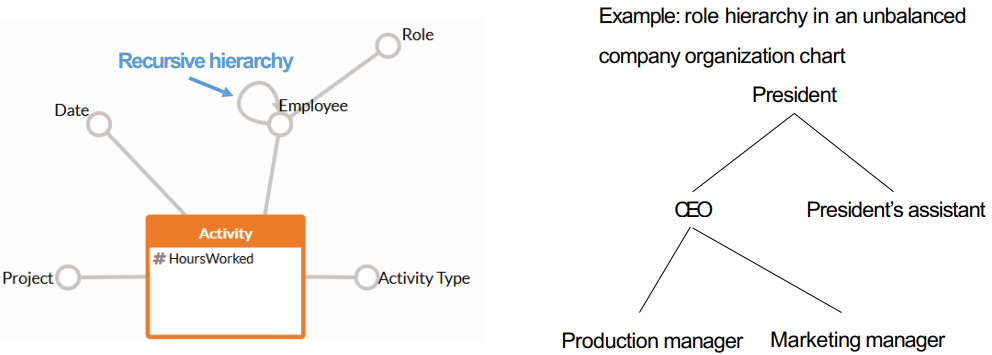
\includegraphics[scale=0.7]{images/DFM_recursive_hierarchies.png}
    \end{figure}
\end{itemize}

\paragraph{Logical Design}
The \textit{\textbf{logical design phase}} defines the data structures (e.g., set of tables and relationships between tables) that represent data marts according to the preselected logical model and optimizes performance by fine tuning these structures.

The logical design phase includes a set of steps that, starting from the conceptual schema, make it
possible to define the logical schema of a data art. Three main steps to implement a logical schema in a relational DBMS:
\begin{itemize}
    \item Translating fact schemata into logical schemata: mainly star or snowflake schemata.
    \item Materializing views: set of secondary view that aggregate primary view data to improve query performance.
    \item Fragmenting fact tables vertically and horizontally.
\end{itemize}

\paragraph{Star schema}
A star schema is characterized by fact tables and dimension tables. A fact table contains all the measures and descriptive attributes linked to a act. A dimensional table is created for each dimension and it includes all the hierarchy attributes [Figure \ref{figStarSchema}].

\paragraph{Snowflake schema}
A star schema variant with dimension tables partially normalized [Figure \ref{figSnowflakeSchema}].
\newpage

\begin{figure}[ht!]
    \centering
    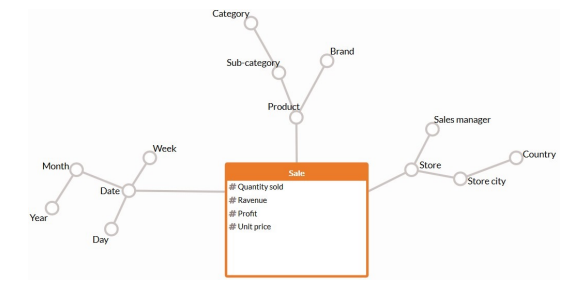
\includegraphics[scale=1.1]{images/DFM_star_schema_1.png}
    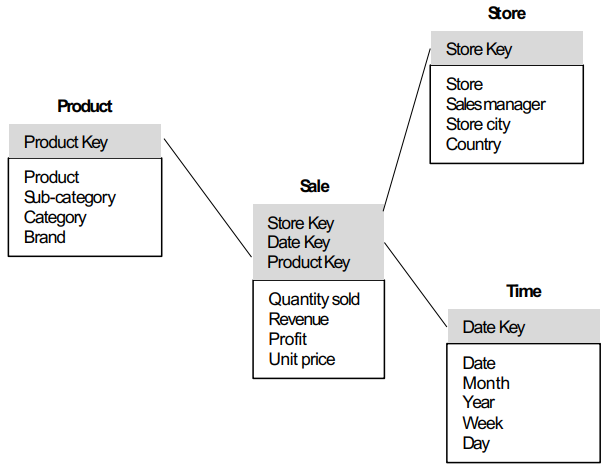
\includegraphics[scale=0.7]{images/DFM_star_schema_2.png}
    \caption{Star Schema}
    \label{figStarSchema}
\end{figure}

\begin{figure}[ht!]
    \centering
    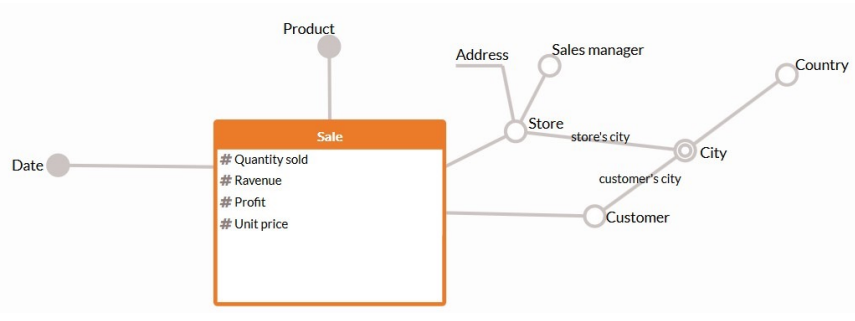
\includegraphics[scale=0.7]{images/DFM_snowflake_schema_1.png}
\end{figure}
\newpage

\begin{figure}[ht!]
    \centering
    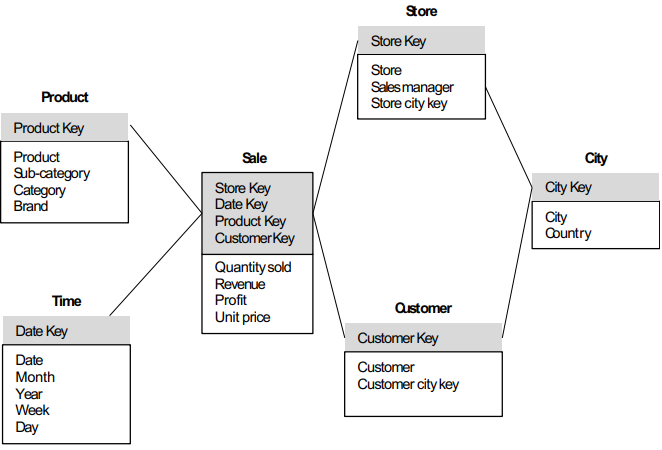
\includegraphics[scale=0.7]{images/DFM_snowflake_schema_2.png}
    \caption{Snowflake Schema}
    \label{figSnowflakeSchema}
\end{figure}

\section{Data Lake}

The down side of data warehousing systems is that they can store only structured data and require a predefined schema. Hence, there are a lot of data that are not used for any business process and they need to be stored somewhere.
\begin{quote}
    \textit{"The storage environments of EMEA organizations consist of 54\% dark data, 32\% redundant, obsolete and trivial data and 14\% business-critical data. By 2020, this can add up to \$891 billion in storage and management costs that can otherwise be avoided."} [sources: Wikipedia and Datamation].
\end{quote}

The solution is to use a \textit{\textbf{Data Lake}}, which is a \textit{centralized repository} that allows you to store a vast amount of data in its \textbf{natural/raw format}, usually \textit{object blobs} or \textit{files}. Two of the keypoints of this approach are the following:
\begin{itemize}
    \item \textbf{Flexibility:} data lakes support various types of data, including structured data from relational databases, semi-structured data like JSON or XML, and unstructured data such as text documents, images, videos, and log files.
    \item \textbf{Schema-on-read:} 
\end{itemize}